\documentclass[11pt]{article}
\usepackage{amsmath,amsthm, amssymb, latexsym,bm}
\usepackage{bbm}
\usepackage{algorithm}% http://ctan.org/pkg/algorithm
\usepackage{algorithmic}
\newcommand{\numpy}{{\tt numpy }}    % tt font for numpy
\usepackage{graphicx}

\usepackage{listings}
\usepackage{xcolor}
\definecolor{codegreen}{rgb}{0,0.6,0}
\definecolor{codegray}{rgb}{0.5,0.5,0.5}
\definecolor{codepurple}{rgb}{0.58,0,0.82}
\definecolor{backcolour}{rgb}{0.95,0.95,0.92}
\lstdefinestyle{mystyle}{
    backgroundcolor=\color{backcolour},
    commentstyle=\color{codegreen},
    keywordstyle=\color{magenta},
    numberstyle=\tiny\color{codegray},
    stringstyle=\color{codepurple},
    basicstyle=\ttfamily\footnotesize,
    breakatwhitespace=false,
    breaklines=true,
    captionpos=b,
    keepspaces=true,
    numbers=left,
    numbersep=5pt,
    showspaces=false,
    showstringspaces=false,
    showtabs=false,
    tabsize=2
}
\lstset{style=mystyle}


\topmargin -.5in
\textheight 9in
\oddsidemargin -.25in
\evensidemargin -.25in
\textwidth 7in

\begin{document}

% ========== Edit your name here
\author{Bruce Chappell}
\title{MAT 4110 Obligatory Assignment 1}
\maketitle

\medskip

% ========== Begin answering questions here
\begin{enumerate}
\section{Introduction}
In this assignment I will study the implementation of QR Factorization and
Cholesky factorization as methods to solve the system:
\begin{equation}
    \label{norm}
    \bm{A \beta = y}
\end{equation}
Where $\bm{A}$ is a matrix of form:
\begin{equation}
    \bm{A} =
    \begin{bmatrix}
        1 & x_{0}^1 & x_{0}^2 & \dots  & x_{0}^{m-1} \\
        1 & x_{1}^1 & x_{1}^2 & \dots  & x_{1}^{m-1} \\
        \vdots     & \vdots  & \vdots & \ddots & \vdots \\
        1 & x_{n-1} & x_{n-1}^2   & \dots  & x_{n-1}^{m-1}
    \end{bmatrix}
\end{equation}
The vector $\bm x$ contains even spaced elements and the vector $\bm y$ is generated by a polynomial function using $\bm x$ as an argument and is possibly noisy.
\\
\\
\section{QR Factorization}
To begin, I used the QR factorization function from \numpy  to factor $\bm A$
into the orthogonal matrix $\bm Q \in \mathbb{R}^{n\times m}$ and the upper triangular matrix $\bm R \in \mathbb{R}^{m\times m}$ resulting in:
\begin{equation}
    \bm{Q R \beta = y}
\end{equation}
Due to orthogonality, $\bm Q^T \bm Q = \mathbbm 1$. Multiplying by $\bm Q^T$ gives:
\begin{equation}
    \bm{R \beta = Q^T y = y^{*}}
\end{equation}
Which can be easily solved by performing back substitution on $\bm R$ shown by the pseudo code below:
\begin{algorithm}
  \begin{algorithmic}[]
    \FOR{$i \in \{n-1,\dots,0\}$}
      \FOR{$j \in \{n-1,\dots,i-1\}$}
        \STATE $y^{*}[i]= y^{*}[i] - \beta[j]\bm R[i,j]$
      \ENDFOR\\
      $\beta[i] = y^{*}[i]/\bm R[i,i]$
    \ENDFOR
  \end{algorithmic}
\end{algorithm}\\

$\bm \beta$ can then be multiplied to the design matrix to obtain the linear regression predicted values of $\bm y$:
\begin{equation}
    \bm{ A \beta  = y_{predict}}
\end{equation}

\section{Cholesky Factorization}
This method solves equation \ref{norm} by factoring a symmetric positive definite matrix $\bm B \in \mathbb{R}^{n\times n}$  into $\bm L \bm L^T$ where $\bm L $ is a lower triangular matrix. Since our design matrix $\bm A$ is in $\mathbb{R}^{n\times m}$ equation \ref{norm} becomes:
\begin{equation}
    \bm{A^T A \beta = A^T y}
\end{equation}
\begin{equation}
    \bm {A^{*} \beta = A^T y}
\end{equation}
We now perform cholesky factorization on the matrix $\bm A{*}$ where the elements of $\bm L$ are computed by the following equations:
\begin{equation}
    l_{kk} = \sqrt{a^{*}_{kk} - \sum_{j=1}^{k-1} l_{kj}^2}
\end{equation}\\
\begin{equation}
    l_{ik} = \frac{1}{l_{kk}}(a^{*}_{ik} - \sum_{j=1}^{k-1} l_{ij}l_{kj})
\end{equation}
The system now becomes:
\begin{equation}
    \bm{L L^T \beta = A^T y = y^{*}}
\end{equation}
We can define $\bm L^T \bm \beta$ as a new unknown vector $\bm g$ and use forward substitution to solve equation 11 for $\bm g$:
\begin{equation}
    \bm{L g = y^{*}}
\end{equation}
And back substitution to solve for $\bm \beta$:
\begin{equation}
    \bm{L^T \beta = g}
\end{equation}
For forward substitution I used to following pseudo code:
\begin{algorithm}
  \begin{algorithmic}[]
    \FOR{$i \in \{0,\dots,n-1\}$}
      \FOR{$j \in \{0,\dots,i-1\}$}
        \STATE $y^{*}[i]= y^{*}[i] - g[j]\bm L[i,j]$
      \ENDFOR\\
      $g[i] = y^{*}[i]/\bm L[i,i]$
    \ENDFOR
  \end{algorithmic}
\end{algorithm}\\
$\bm y_{predict}$ can now be created in the same way as it was with QR factorization.
\section{Plots}
Using two sets of noisy data generated by two different polynomials, both QR and Cholesky factorization were used to to produce fits to the data. Their results for these data sets were identical. Fits were made with degree $m = 3$ and $m = 8$.\\
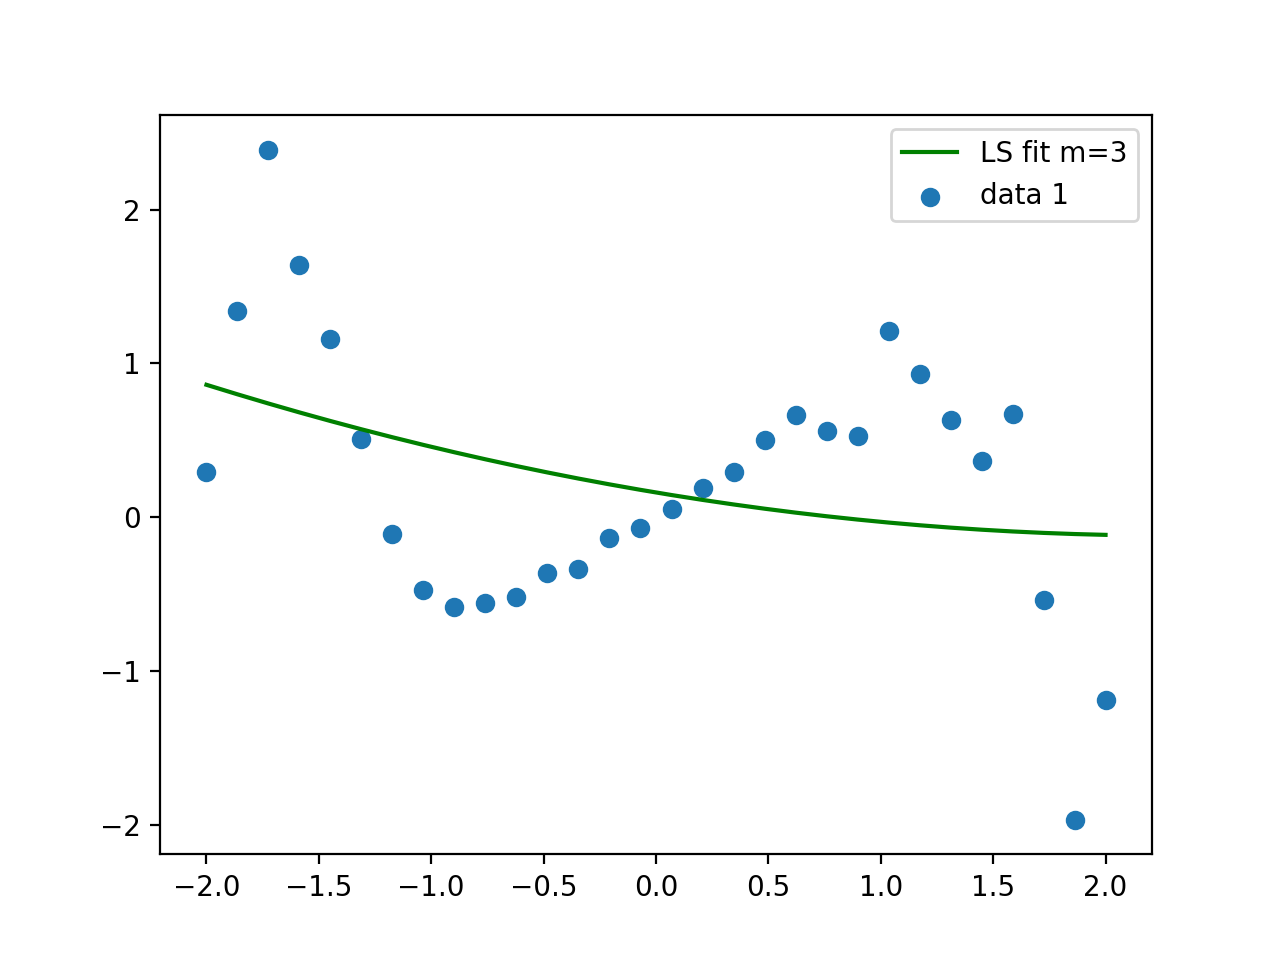
\includegraphics[scale=0.5]{data1_m3.png}
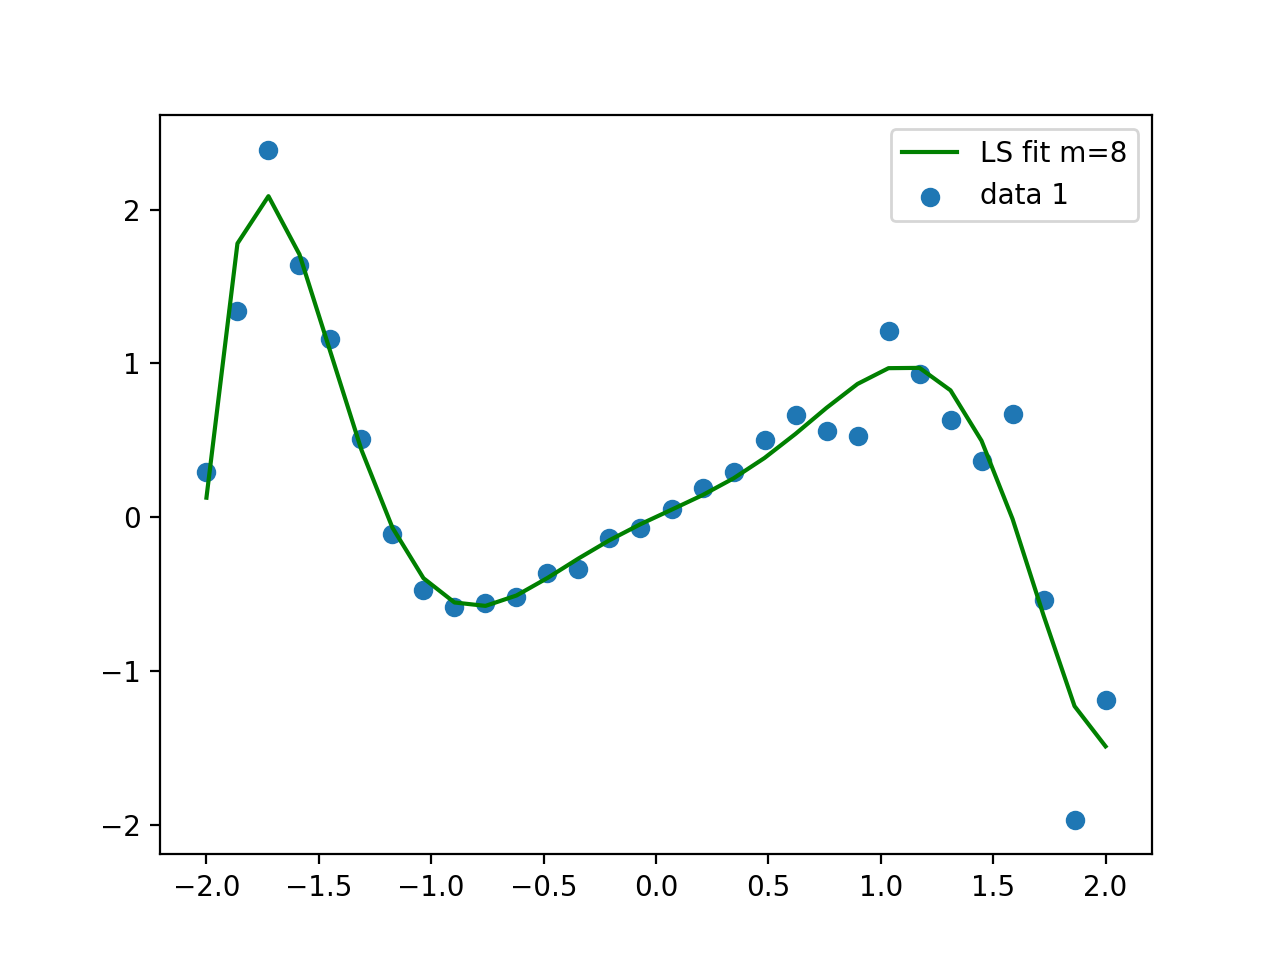
\includegraphics[scale=0.5]{data1_m8.png}\\
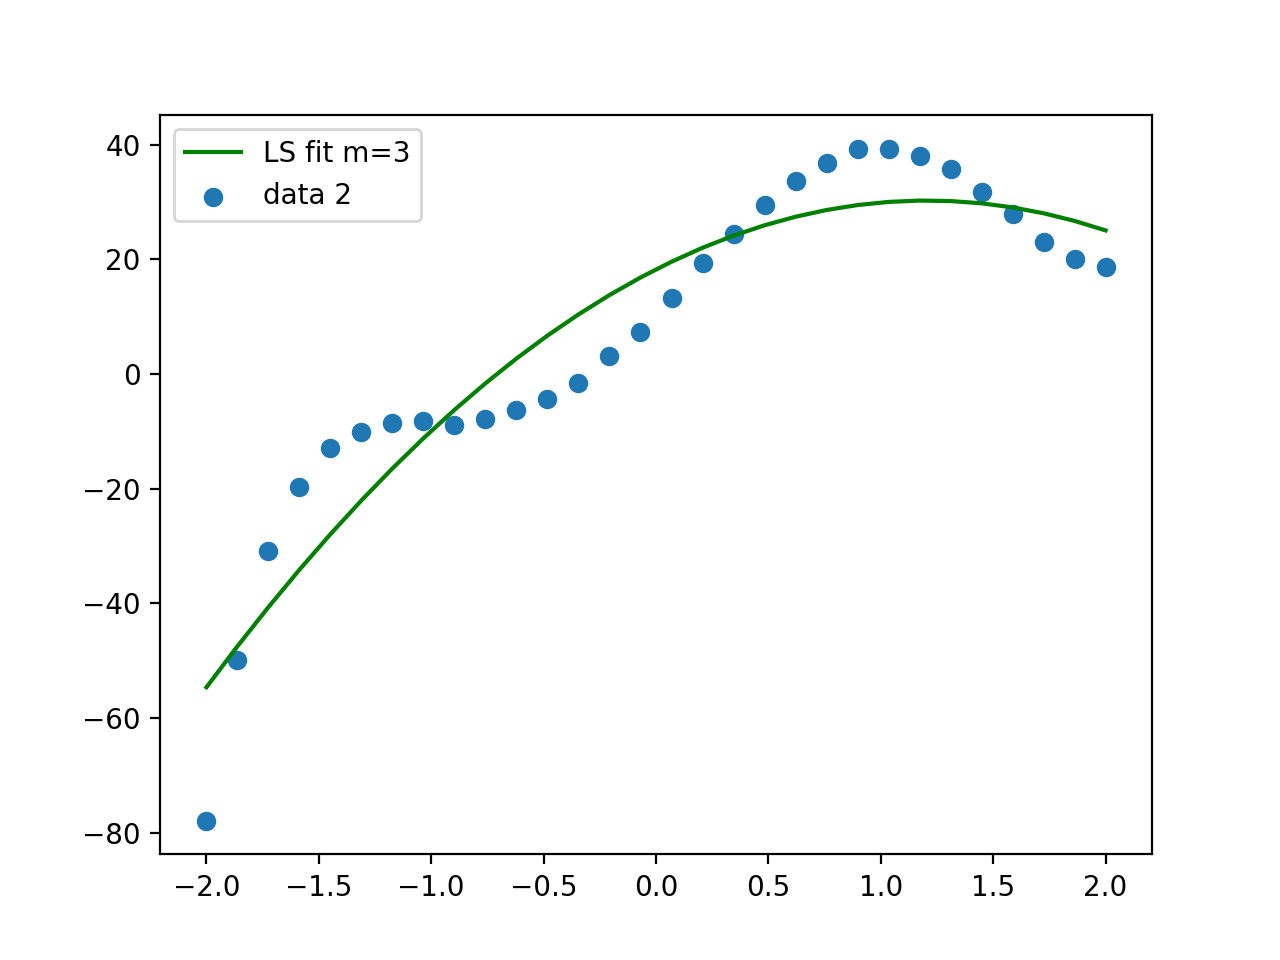
\includegraphics[scale=0.5]{data2_m3.png}
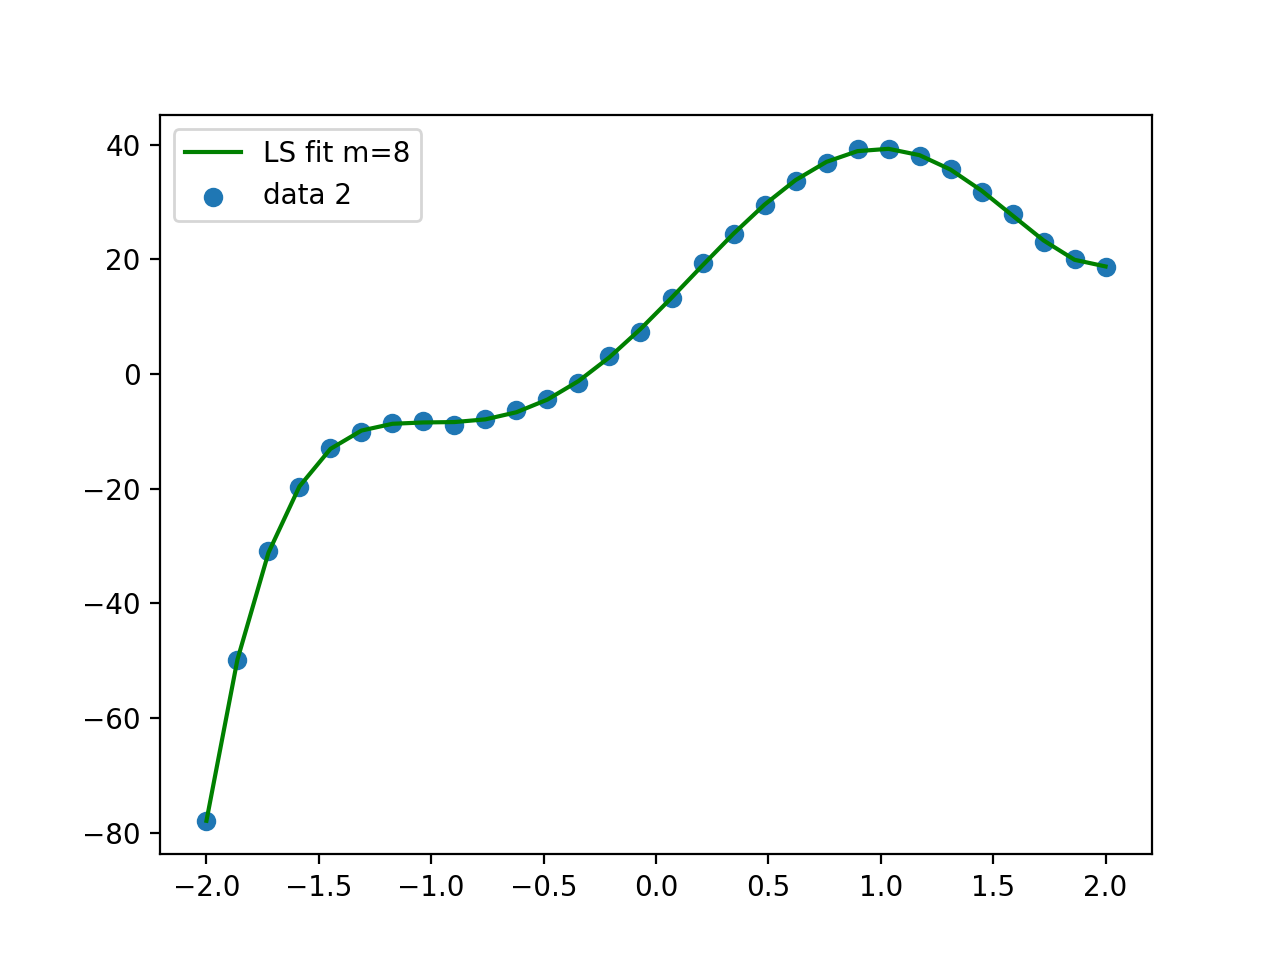
\includegraphics[scale=0.5]{data2_m8.png}\\
For this exercise, I found that QR and Cholesky factorization provided the same results for fitting the data. However, in cases where the data results in a poorly conditioned design matrix QR factorization is a better choice. Cholesky factorization requires taking the square root of a diagonal element of $\bm A^{*}$ which results in a loss of precision greater than normal arithmetic operations.  Additionally, Cholesky factorization requires both forward and backward substitution. If an element on the diagonal of $\bm L$ is close to zero this can create stability problems since $\bm L[i,i]$ is used in the denominator in the algorithm. This would happen in the Cholesky algorithm twice, and only once in the QR algorithm. Below I have attached the code I wrote to generate the data and solve the linear systems.
\end{enumerate}
\begin{lstlisting}[language=Python]
import numpy as np
np.random.seed(1)

def data_set_one(n, start, stop, eps):

    x = np.linspace(start, stop, n)
    r = np.random.rand(n)*eps
    y = x * (np.cos(r + 0.5*x**3) + np.sin(0.5*x**3))
    return x, y

def data_set_two(n, start, stop, eps):
    x = np.linspace(start, stop, n)
    r = np.random.rand(n)*eps
    y = 4*x**5 - 5*x**4 - 20*x**3 + 10*x**2 + 40*x + 10 + r
    return x, y

def designmatrix(x, order):
    mat = np.zeros((len(x),order))
    mat[:,0] = 1
    for i in range(1,order):
        mat[:,i] = x**i
    return mat

def QRsolve(X, y):

    Q, R = np.linalg.qr(X)
    ystar = Q.T @ y

    n = len(ystar)
    beta = np.zeros(n)
    for i in range(n-1, -1, -1):
        tmp = ystar[i]
        for j in range(n-1, i, -1):
            tmp -= beta[j]*R[i,j]
        beta[i] = tmp/R[i,i]
    ypredict = X @ beta
    return ypredict

def cholesky(A):

    A = np.array(A)
    n = A.shape[0]
    L = np.zeros((n,n))

    for row in range(n):
        for col in range(row+1):
            tmp_sum = np.dot(L[row,:col], L[col,:col])
            if (row == col):
                L[row, col] = np.sqrt(A[row,row] - tmp_sum)
            else:
                L[row,col] = (1.0 / L[col,col]) * (A[row,col] - tmp_sum)
    return L

def cholesky_solve(X, y):

    L = cholesky(X.T @ X)
    n = L.shape[0]
    y_1 = X.T @ y

    g = np.zeros(n)
    for i in range(0, n):
         s = y_1[i]
         for j in range(0,i):
              s = s - L[i,j]*g[j]
         g[i] = s / L[i,i]
    beta = np.zeros(n)
    for i in range(n-1, -1, -1):
        tmp = g[i]
        for j in range(n-1, i, -1):
            tmp -= beta[j]*L.T[i,j]
        beta[i] = tmp/L.T[i,i]
    fit = X @ beta
    return fit

\end{lstlisting}


\end{document}
